\documentclass[twoside]{article}

\usepackage{amsfonts}
\usepackage{amsthm}
\usepackage{amsmath}
\usepackage{amssymb}
\usepackage{upgreek}
\usepackage[cm]{fullpage}
%%\usepackage{algorithmic}
%%\usepackage{algorithm} % must read after hyperref
\usepackage[colorlinks={true}, citecolor=blue, linkcolor=blue]{hyperref}       % hyperlinks
\usepackage{algpseudocode}
\usepackage{bbm}
\usepackage{bm}
\usepackage{graphicx}
\graphicspath{{./img/}}
\newtheorem{proposition}{Proposition}

%% \usepackage{array}
%% \usepackage{comment,array,wasysym}
%% \usepackage{graphicx,color,colortbl}

%% % \usepackage{mathptmx} % Use Times as default text font, and provide maths support.  I hate what it does to mathcal so I comment it out
%% % \usepackage{mathtools}
%% % \usepackage{multimedia}
%% % \usepackage{subfigure}
%% %\usepackage{ulem} % for strikethrough \sout
%% \usepackage[normalem]{ulem} % for strikethrough \sout, but avoid the annoying underline in \emph



%% % 
%% % \usepackage[utf8x]{inputenc}
%% % \usepackage{default}

%% % AISTATS sty file doesn't play nicely with caption and subcaption pkgs
%% % \usepackage{caption} 
%% %\usepackage{subcaption}

%% \usepackage{caption}
%% \DeclareCaptionType{copyrightbox}  % Without this, the AISTATs sty creates some clash
%% \usepackage{subcaption}


%% \usepackage{ifthen}
%% \usepackage{enumerate}


%% % 
%% % 
%% %         
%% % \usepackage{yhmath}  % I want really wide tilde. Oren Freifeld, 05/19/2013       




%% %% ICML PACKAGES %%
%% %% \usepackage{ellipsis}

%% %% \usepackage{multirow}

%% %% % Recommended, but optional, packages for figures and better typesetting:
%% %% \usepackage{microtype}
%% %% \usepackage{graphicx}
%% %% % \usepackage{subfigure}
%% %% \usepackage{booktabs} % for professional tables

%% %% % hyperref makes hyperlinks in the resulting PDF.
%% %% % If your build breaks (sometimes temporarily if a hyperlink spans a page)
%% %% % please comment out the following usepackage line and replace
%% %% % \usepackage{icml2018} with \usepackage[nohyperref]{icml2018} above.
%% %% \usepackage{hyperref}

%% %% % Attempt to make hyperref and algorithmic work together better:
%% %% \newcommand{\theHalgorithm}{\arabic{algorithm}}


%% %
%% % Commenting macros
%% %
%% \newcommand{\BLUE}[1]{{{\color{blue}{#1}}}}      
\newcommand{\RED}[1]{{{\color{red}{#1}}}}     
%% \newcommand{\MAGENTA}[1]{{{\color{magenta}{#1}}}}     
%% \definecolor{darkgreen}{rgb}{0,.5,0 }
%% \newcommand{\DARKGREEN}[1]{{{\color{darkgreen}{#1}}}}      
%% \newcommand{\TBD}{\RED{[--TBD--]}}
%% \newcommand{\TODO}[1]{\RED{[--TODO: #1--]}}
%% \newcommand{\BRAINDUMP}[1]{\DARKGREEN{[BRAIN DUMP: #1]}}
%  
%  \newcommand{\OREN}[1]{\RED{[Oren says: #1]}}
% % PICK YOUR COLOR...
\newcommand{\jwf}[1]{\BLUE{<\textbf{JWF}: #1 >}}
% \newcommand{\SUE}[1]{\MAGENTA{[Sue says: #1]}}

% MRF
\newcommand{\pot}{\psi}
\newcommand{\epmarg}{q}
\newcommand{\logpart}{\Phi}

% min / max
\DeclareMathOperator*{\argmax}{arg\,max\;}
\DeclareMathOperator*{\argmin}{arg\,min\;}

% Info Theory Stuff
\newcommand{\KL}[2]{\mathrm{KL}(#1\,\|\,#2)}

%
% List macros
%
\newcommand{\bi}{\begin{itemize}}
\newcommand{\ei}{\end{itemize}}
\newcommand{\deriv}{\mathrm{d}}

\newcommand{\etal}{\textit{et al}}
\newcommand{\FIG}{Fig.~}
%\newcommand{\FIGS}{Figs.~}

 \newcommand{\SEC}{Sec.~}

\newcommand{\eg}{\textit{e.g.}~}
\newcommand{\ie}{\textit{i.e.}~}
\newcommand{\cf}{\textit{c.f.}~}


\newcommand{\EQN}{Eqn.~}
% \newcommand{\EQN}{Equation }
\newcommand{\EQNS}{Eqns.~}
% \newcommand{\EQNS}{Equations }

% Expectation and Probability
\newcommand{\EE}{\ensuremath{\mathbb{E}}}
\newcommand{\PP}{\ensuremath{\mathbb{P}}}


% distributions
\newcommand{\Dir}{\ensuremath{\text{Dirichlet}}}
 
% integers
\newcommand{\ZZ}{\ensuremath{\mathbb{Z}}}
\newcommand{\RR}{\ensuremath{\mathbb{R}}}
\newcommand{\Rtwo}{\ensuremath{\RR^2}}
\newcommand{\Rthree}{\ensuremath{\RR^3}}
\newcommand{\Rn}{\ensuremath{\RR^n}}
% 
%positive integers
\newcommand{\Zplus}{\ensuremath{\ZZ^+}}
%positive reals
\newcommand{\Rplus}{\ensuremath{\RR^+}}


% n by n matrices
\newcommand{\nBynMats}{\ensuremath{\RR^{n \times n}}}
% m by n matrices
\newcommand{\mBynMats}{\ensuremath{\RR^{m \times n}}}
% n by p matrices
\newcommand{\nBypMats}{\ensuremath{\RR^{n \times p}}}
% 2 by 2
\newcommand{\TwoByTwoMats}{\ensuremath{\RR^{2 \times 2}}}
% 3 by 3
\newcommand{\ThreeByThreeMats}{\ensuremath{\RR^{3 \times 3}}}
% 2 by 3
\newcommand{\TwoByThreeMats}{\ensuremath{\RR^{2 \times 3}}}




% \newcommand{\EqualsDef}{\,{\overset{\text{def}}{=}}\,}
\newcommand{\EqualsDef}{\triangleq}


% set notation
% \newcommand{\set}[1]{\ensuremath{{\left\{#1\right\}}}}
\newcommand{\set}[1]{\ensuremath{{\{#1\}}}}


\newcommand{\InnerProduct}[2]{\left\langle #1,#2 \right\rangle}

\newcommand{\norm}[1]{{{\left\|#1\right\|}}}
\newcommand{\sign}[1]{{\mathrm{sign}\left(#1\right)}}


\newcommand{\ellTwoNorm}[1]{\norm{#1}_{\ellTwo}}


\newcommand{\Acal}{\mathcal{A}}
\newcommand{\Bcal}{\mathcal{B}}
\newcommand{\Ccal}{\mathcal{C}}
\newcommand{\Dcal}{\mathcal{D}}
\newcommand{\Ecal}{\mathcal{E}}
\newcommand{\Fcal}{\mathcal{F}}
\newcommand{\Gcal}{\mathcal{G}}
\newcommand{\Mcal}{\mathcal{M}}
\newcommand{\Ncal}{\mathcal{N}}
\newcommand{\Ocal}{\mathcal{O}}
\newcommand{\Pcal}{\mathcal{P}}
\newcommand{\Qcal}{\mathcal{Q}}
\newcommand{\Tcal}{\mathcal{T}}
\newcommand{\Vcal}{\mathcal{V}}
\newcommand{\Wcal}{\mathcal{W}}
\newcommand{\Xcal}{\mathcal{X}}
\newcommand{\Ycal}{\mathcal{Y}}

\newcommand{\MATRIX}[2][cccccccccccccccccccc]{\left[
 \begin{array}{#1}
 #2
 \end{array}
\right]}


\newcommand{\TRACE}{\mathrm{trace}}

\newcommand{\var}[1]{\text{var} \big( #1 \big) }
\newcommand{\cov}[2]{\text{cov} \big( #1,#2 \big)}
\newcommand{\myt}[1]{\widetilde {#1} }

% bold font math 
\bmdefine\balpha{\alpha}
\bmdefine\bbeta{\beta}

\bmdefine\bphi{\phi}


\bmdefine\bb{b}

\bmdefine\bx{x}
\bmdefine\by{y}
\bmdefine\bdotx{\dot{x}}
\bmdefine\bxzero{x_{0}}
\bmdefine\bxone{x_{1}}

\bmdefine\bu{u}

\bmdefine\bv{v}
\bmdefine\br{r}


\bmdefine\bA{A}
\bmdefine\bB{B}

\bmdefine\bS{S}

\bmdefine\bU{U}

\bmdefine\bV{V}
\bmdefine\bX{X}
\bmdefine\bY{Y}


%\bmdefine\balpha{\alpha}

 \newcommand{\Nc}{{N_{c}}}
% \newcommand{\Nc}{N}
\newcommand{\Ne}{{N_{e}}}

% homo coo
\newcommand{\bxh}{\widetilde{\bx}}




\newcommand{\GLn}{\ensuremath{\mathrm{GL(n)}}}
\newcommand{\gln}{\ensuremath{\mathfrak{gl(n)}}}

\newcommand{\GLone}{\ensuremath{\mathrm{GL(1)}}}
\newcommand{\GLtwo}{\ensuremath{\mathrm{GL(2)}}}
\newcommand{\glTwo}{\ensuremath{\mathfrak{gl}(2)}}


% CPA Stuff

\newcommand{\Ac}[1]{A_{c(#1)}}
\newcommand{\Bc}[1]{B_{c(#1)}}

\newcommand{\Vaff}{\Vcal_{\mathrm{aff}}}

\newcommand{\Vpa}{\Vcal_{\mathrm{PA}}}
\newcommand{\Vcpa}{\Vcal_{\mathrm{CPA}}}


\newcommand{\Faff}{\Fcal_{\mathrm{aff}}}

\newcommand{\Fpa}{\Fcal_{\mathrm{PA}}}
\newcommand{\Fcpa}{\Fcal_{\mathrm{CPA}}}

\newcommand{\NSTEPS}{N_{\mathrm{STEPS}}}
\newcommand{\nsteps}{n_{\mathrm{steps}}}


\newcommand{\SigmaPA}{\Sigma_{\mathrm{PA}}}

\newcommand{\SigmaCPA}{\Sigma_{\mathrm{CPA}}}



\newcommand{\Vat}[1]{\bv{(#1)}}
\newcommand{\VatX}{\Vat{\bx}}
\newcommand{\Tat}[2]{T{(#1,#2)}}
\newcommand{\Tinvat}[2]{T^{-1}{(#1,#2)}}
\newcommand{\VatT}[1][t]{\Vat{\Tat{\bx}{#1}}}
% \newcommand{\VatT}[1][t]{\Vat{\Tat{\bx,#1}}}
\newcommand{\VatTinv}[1][t]{\Vat{\Tinvat{\bx}{#1}}}


\newcommand{\IntVatTofX}[1][t]{\int_{0}^{#1}\VatT[\tau]\, d\tau}

\newcommand{\AtimesX}{A{\bxh}}
 

\newcommand{\CpaVatX}{\Ac{\bx}\bxh}
% \newcommand{\CpaVatT}[1][t]{\Ac{\Tat{\bx}{#1}}\widetilde{T}(\bx,#1)}
\newcommand{\CpaVatT}[1][t]{\Ac{\Tat{\bx}{#1}}\widetilde{\Tat{\bx}{#1}}}

\newcommand{\IntCpaVatT}[1][t]{\int_{0}^{#1} \CpaVatT[\tau] \, d\tau}


 

\newcommand{\IntCpaVatTinv}[1][t]{\int_{0}^{#1}  \Ac{\Tinvat{\by}{#1}}\widetilde{\Tinvat{\by}{#1}} \, d\tau}


\newcommand{\CpaVatXasLinComb}{\sum_{j=1}^{d}\alpha_k\Bc{\bx}^{j}\bxh}
\newcommand{\CpaVatTasLinComb}[1][t]{\sum_{j}^{d}\alpha_j\Bc{\Tat{\bx}{#1}}^{j}\widetilde{\Tat{\bx}{#1}}}


\newcommand{\IntCpaVatTLinComb}[1][t]{\int_{0}^{#1}  \CpaVatTasLinComb[\tau] \, d\tau}


% USAGE:
% $\Vat{\bx}$
% $\VatX$
% $\Tat{\bx}{t}$
% $\VatT$
% $\VatT[\tau]$
% $\VatTinv[\tau]$
% $\IntVatTofX$
% $\AtimesX$
% $\Ac{\bx}$
% $\CpaVatX$
% $\IntCpaVatT$
% $\CpaVatXasLinComb$
% $\IntCpaVatTLinComb$



%\newcommand{\VEE}[1]{{#1}^{\vee}}
\newcommand{\VEE}[1]{\mathrm{vec}({#1})}

\newcommand{\HAT}[1]{{#1}^{\wedge}}

 \newcommand{\LCONSTRAINTS}{L_{\mathrm{constraints}}}

% Graph stuff
\newcommand{\parent}{\text{Pa}}
\newcommand{\interventions}{\mathcal{I}}
\newcommand{\alldata}{\mathcal{X}}

% Planning stuff
\newcommand{\actionset}{\mathcal{A}}



%\usepackage{aistats2019}
% If your paper is accepted, change the options for the package
% aistats2019 as follows:
%
\usepackage[accepted]{aistats2019}
%
% This option will print headings for the title of your paper and
% headings for the authors names, plus a copyright note at the end of
% the first column of the first page.

% If you set papersize explicitly, activate the following three lines:
%\special{papersize = 8.5in, 11in}
%\setlength{\pdfpageheight}{11in}
%\setlength{\pdfpagewidth}{8.5in}

% If you use natbib package, activate the following three lines:
\usepackage[round]{natbib}
\renewcommand{\bibname}{References}
\renewcommand{\bibsection}{\subsubsection*{\bibname}}

% If you use BibTeX in apalike style, activate the following line:
%\bibliographystyle{apalike}

\begin{document}

% If your paper is accepted and the title of your paper is very long,
% the style will print as headings an error message. Use the following
% command to supply a shorter title of your paper so that it can be
% used as headings.
%
%\runningtitle{I use this title instead because the last one was very long}

% If your paper is accepted and the number of authors is large, the
% style will print as headings an error message. Use the following
% command to supply a shorter version of the authors names so that
% they can be used as headings (for example, use only the surnames)
%
\runningauthor{J. Pacheco and J.W. Fisher, III}

\twocolumn[

  \aistatstitle{Variational Information Planning for Sequential Decision Making} 
  \aistatsauthor{ Jason Pacheco \And John W. Fisher, III}
  \aistatsaddress{ MIT CSAIL \And MIT CSAIL} ]

\begin{abstract}  
  We consider the setting of sequential decision making where, at each
  stage, potential actions are evaluated based on expected reduction
  in posterior uncertainty, given by mutual information (MI).  As MI
  typically lacks a closed form, we propose an approach which
  maintains variational approximations of, both, the posterior and MI
  utility.  Our planning objective extends an established variational
  bound on MI to the setting of sequential planning.  The result,
  variational information planning (VIP), is an efficient method for
  sequential decision making.  We further establish convexity of the
  variational planning objective and, under conditional exponential
  family approximations, we show that the optimal MI bound arises from
  a relaxation of the well-known exponential family moment matching
  property.  We demonstrate VIP for sensor selection, experiment
  design, and active learning, where it meets or exceeds methods
  requiring more computation, or those specialized to the 
  task.
\end{abstract}

\section{Introduction}
Bayesian machine learning research has paid much attention to the
development of posterior inference algorithms, yet comparatively
little attention to methods for decision making based on the results
of inference.  In this paper we explore sequential decision making
based on information theoretic quantities.  Specifically, we introduce
efficient methods for \emph{information planning}, where decisions are
generated by maximizing the mutual information (MI)
utility~\citep{WilliamsThesis}.

Our setting resembles Bayesian experiment design~\citep{lindley56},
where experiments are chosen to minimize uncertainty over a quantity
of interest.  MI has long been used as a design utility in this
setting~\citep{blackwell50, bernardo79a}.  Unlike experiment design,
which typically assumes the cost of a measurement dominates that of
inference, our focus is on high throughput sequential decision
systems.  Where the former relies on Markov chain Monte Carlo (MCMC),
we present a comprehensive approach to inference and planning based on
efficient variational approximations.

Our approach, which we call variational information planning (VIP),
maintains a series of variational approximations to the posterior and
MI utility.  For the planning stage, VIP extends a lower bound of
MI~\citep{agakov2004algorithm} to the sequential setting.  The bound
is optimized over an auxiliary distribution approximating the expected
posterior.  We demonstrate that VIP yields a convex optimization for
exponential family auxiliary models, leading to efficient planning.
We establish optimality conditions for the natural parameters of this
family, and show that they are a relaxation of the well known moment
matching conditions.

%% Our setting differs from both Bayesian experimental design and RL in a
%% number of ways.  Traditional experiment design typically assumes the
%% cost of observation outweighs that of inference, and thus relies on
%% Markov chain Monte Carlo (MCMC) methods for inference.  MI is then
%% estimated over samples, resulting in estimator bias with slow
%% convergence~\citep{zheng2018robust, rainforth2018nesting}.  In
%% comparison to RL planning, our utility of interest is thus purely
%% exploratory, thus contrasting with the exploration-exploitation
%% trade-off common in RL planning~\citep{sutton1998reinforcement}.
%% Other differences with RL include the use of a structured statistical
%% model and representation of latent variables.

%% Statistical experiment design typically presumes that the cost of
%% experiments, or the cost of observation, far exceed the cost of
%% computation, and therefore rely on Markov chain Monte Carlo (MCMC)
%% methods for computation.  Such an approach is impractical for
%% high-throughput decision systems.  Moreover, Monte Carlo estimates of
%% MI have been shown to be biased due to the use of nested Monte Carlo
%% estimation, and that the rate of bias decay can be
%% slow~\citep{zheng2018robust, rainforth2018nesting}.

Despite good predictive accuracy, variational approximations of
posterior uncertainty can be poor~\citep{giordano2015linear,
turner2011two}.  Thus, a naive variational approach will tend to yield
poor planning decisions.  We address these issues by defining a class
of auxiliary distributions that, when conditioned on future
observations, define exponential families.  This set allows arbitrary
nonlinear dependence on the observation variable, and is thus strictly
larger than the set of jointly exponential family models.

In our experiments we demonstrate that VIP is sufficiently flexible to
apply in a variety of problem instances such as nonlinear target
tracking in a sensor network, experiment design, and active learning.
Moreover, VIP meets or exceeds the accuracy of methods based on exact
inference, MCMC requiring more computation, or specialized variational
approximations. 

%% and maximize a
%% well-known lower bound of MI resulting from Gibbs'
%% inequality~\citep{agakov2004algorithm}.  The bound is maximized over
%% an auxiliary model, which is strictly more expressive than the
%% exponential family posterior approximation, thus allowing for better
%% representations of uncertainty.  Moreover, we show that when this
%% class of models is conditionally in the exponential family, the
%% resulting optimization problem is convex.  We also show connections to
%% MI approximation based on moment matching operations, and that it is
%% equivalent to our approach in some restricted settings.  Finally, we
%% demonstrate effectiveness on a variety of problems including nonlinear
%% target tracking in a sensor network, gene regulatory network
%% inference, and active learning in the labeled LDA model (LLDA).




\section{Sequential Information Planning}
Consider a model of latent variables $x$ and observations $\Ycal_{t-1}
= \{y_1,\ldots,y_{t-1}\}$.  At each time $t-1$ a discrete
\emph{action} $a_{t-1} \in \{1,\ldots,A\}$ parameterizes the
likelihood, denoted \mbox{$p_{a_{t-1}}(y_{t-1} \mid x)$}.  Let
$\Dcal_{t-1} = \{\Ycal_{t-1},\Acal_{t-1}\}$ be the set of observations
and chosen actions \mbox{$\actionset_{t-1} =
\{a_1,\ldots,a_{t-1}\}$} at time $t-1$.  The posterior is then,
\begin{equation}\label{eq:conditional_indep_joint}
  p(x\mid \Dcal_{t-1}) \propto
    p(x) \prod_{i=1}^{t-1} p_{a_i}(y_i \mid x)
\end{equation}
The goal of sequential information planning is to choose the sequence
of actions $\Acal$ that minimize entropy of the
posterior~\eqref{eq:conditional_indep_joint}.  Specifically, at time
$t$, an action $a_t$ is selected to maximize the posterior mutual
information,
\begin{align}\label{eq:post_mi}
  a_t^{*} &= \argmax_a I(X;Y_t \mid \Dcal_{t-1}) \notag \\
          &= \argmax_a H(X\mid \Dcal_{t-1}) - H_a(X \mid Y_t, \Dcal_{t-1})
          %% &= \argmax_a H(X\mid \Dcal_{t-1}) + H_a(Y_t\mid \Dcal_{t-1})
          %% - H_a(X, Y_t \mid \Dcal_{t-1}).
\end{align}
Once an action is selected, new observations are drawn from the
appropriate likelihood model $y_t \sim p_{a_t}(\cdot \mid x)$ and the
posterior is updated.

%% We assume in \EQN\eqref{eq:info_plan_obj} that the marginal
%% entropy \mbox{$H(X\mid \Dcal)$} is invariant to future actions, and
%% thus can be ignored for planning.

Calculating the posterior MI in \EQN\eqref{eq:post_mi} is complicated
for two reasons.  First, the entropy terms involve expectations under
the posterior distribution~\eqref{eq:conditional_indep_joint}.
Second, calculating the conditional entropy $H(X\mid Y, \Dcal)$ requires
evaluation of the posterior predictive distribution $p(y\mid \Dcal)$
as in,
\[
  H(X\mid Y, \Dcal) = \EE\left[
    - \log \frac{p(x,y\mid \Dcal)}{ p(y\mid \Dcal) } \right],
\]
where we have dropped explicit indexing on time.  One approach is to
estimate this over samples \mbox{$\{y^i_t\} \sim
p_a(y\mid \Dcal_{t-1})$}.  The resulting empirical plug-in estimator
of MI is,
%% \begin{equation}\label{eq:emp_mi}
%%   \hat{I}_a = \frac{1}{N} \sum_{i=1}^N \log \frac{ p_a(y_t^i \mid x^i)
%%   }{ \frac{1}{M} \sum_{j=1}^M p_a(y_t^i \mid x^{ij}) }.
%% \end{equation}
\begin{equation}\label{eq:est_margent}
  \hat{I}_a \approx - \frac{1}{N} \sum_{i=1}^N \log \frac{
    p_a(y_t^i\mid x^i) }{\frac{1}{M}
        \sum_{j=1}^M p_a(y_t^i \mid x^{ij})}.
\end{equation}
Independent samples $\{x^{ij}\}_{j=1}^M \sim p(x \mid \Dcal_{t-1})$
are required for each action, and observation sample, to ensure
estimates are independent, thus increasing sample complexity.  While
the estimator~\eqref{eq:est_margent} is consistent, it is biased.
Moreover, bias is known to decay slowly~\citep{zheng2018robust,
rainforth2018nesting}.

%% %% \mbox{$I(X;Y_t \mid \Ycal_{t-1}, \Acal_{t-1})$}. 
%% %% \begin{align}
%% %%   a_t^{*} &= \argmax_a I_a(X;Y_t \mid \Ycal_{t-1}, \Acal_{t-1}) \\
%% %%     &= H(X\mid \Ycal_{t-1}, \Acal_{t-1}) - H_a(X, Y_t \mid
%% %%       \Ycal_{t-1}, \Acal_{t-1}). \notag
%% %% \end{align}
%% \begin{equation}
%%   a_t^{*} = \argmax_a H(X) + H_a(Y_t) - H_a(X, Y_t). \notag
%% \end{equation}


\section{Variational Information Planning}\label{sec:varplan}
\begin{figure*}[t]
  \centering
  \begin{tabular}{cccc}
    \hspace{-9mm}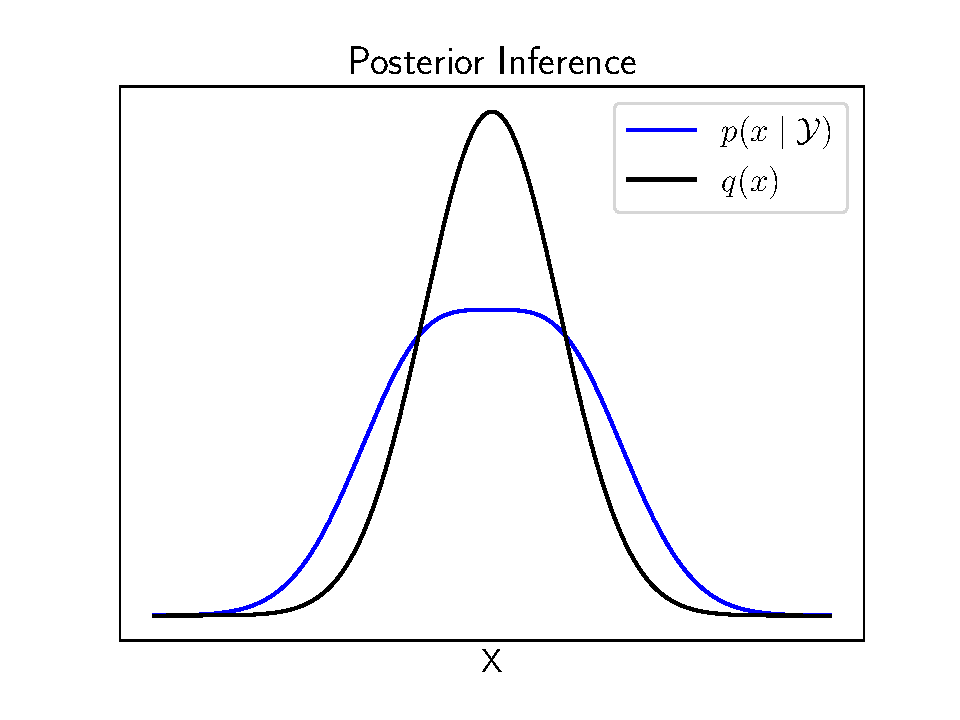
\includegraphics[width=0.29\textwidth]{inf_approx} &
    \hspace{-9mm}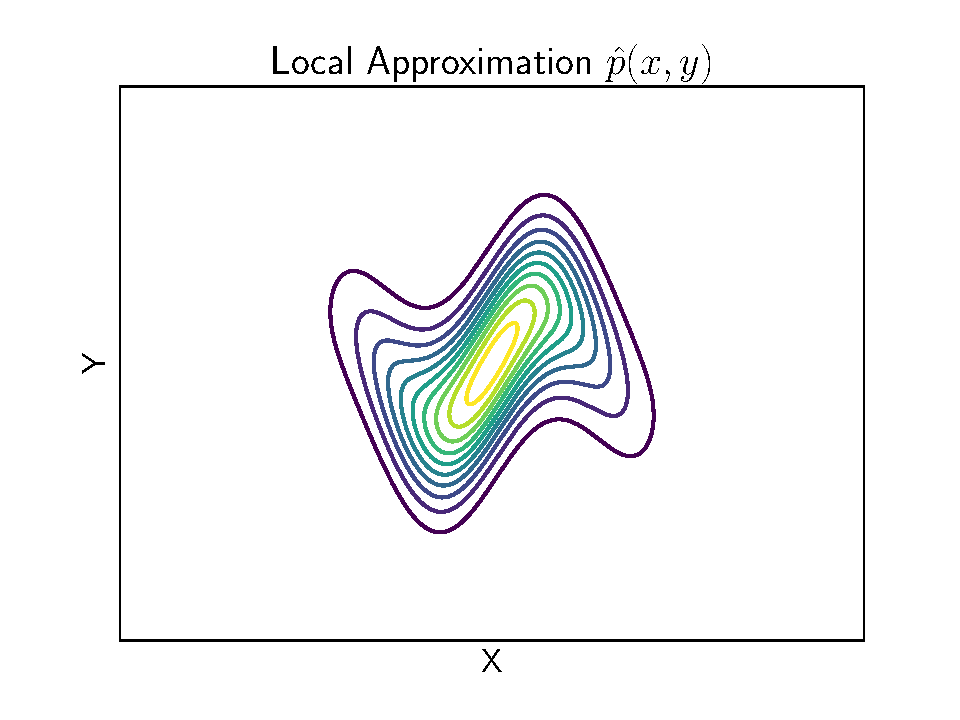
\includegraphics[width=0.29\textwidth]{augmented_dist} &
    \hspace{-9mm}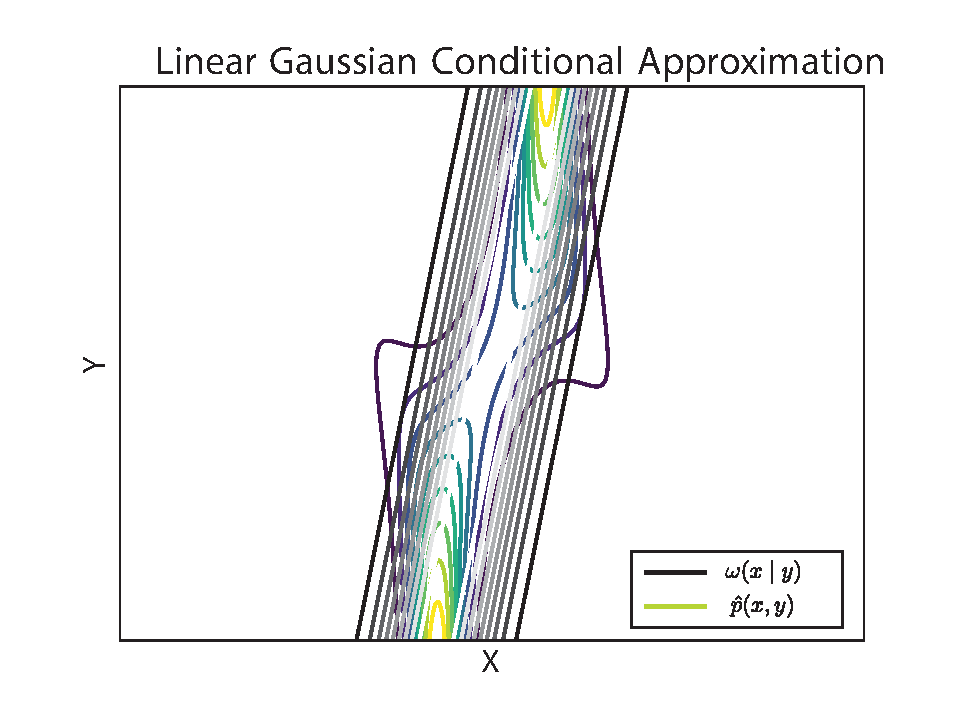
\includegraphics[width=0.29\textwidth]{linear_approx} &
    \hspace{-9mm}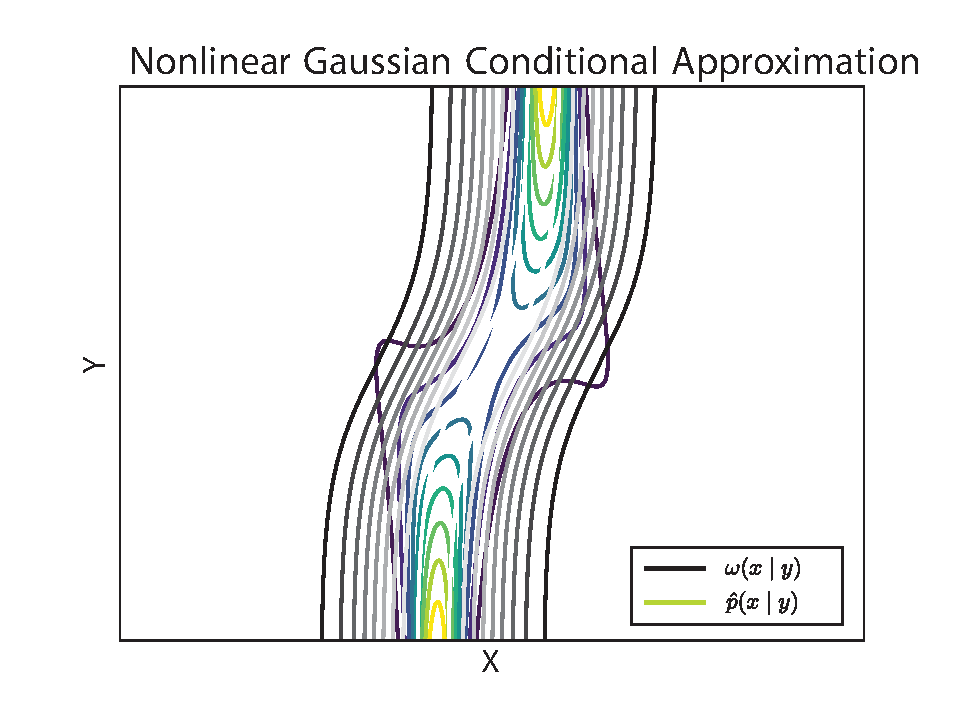
\includegraphics[width=0.29\textwidth]{nonlinear_approx}
  \end{tabular}

  \caption{\small \textbf{Distributional approximations.} \emph{Left:}
  Given observations $\Ycal$ the posterior is approximated with a
  tractable family $q(x) \approx p(x\mid \Ycal)$.  \emph{Center-Left:}
  To consider a new observation $y$, a local approximation is formed
  $\hat{p}(x,y) = q(x) p(y \mid x)$ using the forward model $p(y\mid
  x)$.  \emph{Center-Right:} VIP optimizes a lower bound on MI
  w.r.t.~a distribution $\omega(x\mid y)$ approximating the
  conditional $\hat{p}(x\mid y)$. We use a linear Gaussian
  approximation in this case.  \emph{Right:} Directly parameterizing
  the conditional $\omega(x\mid y)$ allows nonlinear functions of the
  conditioning variable $y$, allowing for better approximations and
  tighter bounds.}

  \label{fig:approx}
\end{figure*}

For any valid distribution $\omega(x\mid y)$, the following is a lower
bound on MI,
\begin{equation}\label{eq:varmi}
  I(X;Y) \geq H(X) + \EE_p[ \log \omega(X\mid Y) ].
\end{equation}
This well-known bound is a result of Gibbs' inequality.  It has been
independently explored for channel coding~\citep{agakov2004algorithm},
reinforcement learning~\citep{mohamed2015variational}, and feature
selection~\citep{gao2016variational, chen2018learning}.
Unfortunately, we cannot directly apply the bound in
\EQN\eqref{eq:varmi} since, in our setting, it involves posterior
expectations.

In this section we describe one approach to bounding MI for sequential
planning, which involves a series of approximations.  First, given
past observations $\Ycal$, we approximate the posterior
\mbox{$q(x)\approx p(x\mid \Ycal)$} with a tractable distribution.
Then, a local approximation is formed \mbox{$\hat{p}(x,y) \approx
  p(x,y\mid \Ycal)$} for some future observation $y$.  Finally, we
optimize the auxiliary distribution $\omega(x\mid y)$, which tightens
a lower bound of MI under $\hat{p}(\cdot)$.  See \FIG\ref{fig:approx}
for an illustration.

\subsection{Conditionally Independent Observations}

We begin with the simple model in
\EQN\ref{eq:conditional_indep_joint}, where observations $y$ are
independent conditioned on latent $x$.  Having performed actions
$\Acal_{t-1}$, and observed measurements $\Ycal_{t-1}$, assume that we
have a tractable approximation of the posterior \mbox{$q(x) \approx
  p(x \mid \Ycal_{t-1}, \Acal_{t-1})$}.  We then form a local
approximation of the distribution over a future measurement at time
$t$,
\begin{equation}\label{eq:local_approx}
  \hat{p}_{a}(x,y_t) \equiv q_{t-1}(x) p_{a}(y_t \mid x).
\end{equation}
Here, $p_{a}(y_t \mid x)$ is the true likelihood under the
hypothesized action $a$.  The distribution $\hat{p}(\cdot)$ is
analogous to the \emph{augmented distribution} at each stage of EP
inference, which we will exploit in the next section.  We can then
bound the MI under $\hat{p}(\cdot)$ as,
\begin{equation}\label{eq:varmi_approx}
  H_{\hat{p}}(X) + \max_{a, \,\omega}  \;\EE_{\hat{p}_a}\left[ \log \omega(X \mid Y_{t+1})
  \right].
\end{equation}
We have moved the marginal entropy outside the optimization since it is
constant in this model, and so can be ignored for planning.  The bound
can be evaluated in parallel for a discrete set of actions
$1,\ldots,A$.

\FIG\ref{fig:approx} illustrates the role of each approximation in a
single planning stage, and how the approximations relate to the target
distributions.  To be clear, \EQN\eqref{eq:varmi_approx} bounds mutual
information w.r.t.~the local approximate distribution
$\hat{p}(\cdot)$, not MI under the true posterior.  To ensure that MI
under $\hat{p}(\cdot)$ is a reliable surrogate for posterior MI,
$q(x)$ must accurately approximate the posterior.

\subsection{Annotation Models}\label{sec:annotation}

The conditionally independent model of the previous section is a
simple model chosen for illustrative purposes.  We now consider a
different, more complicated distribution, often arising in active
learning~\citep{settles2012active}.  More specifically, consider a
joint distribution over latent $x$, data $\{z_d\}_{d=1}^D$ which are
fixed, and annotations $\{y_d\}_{d=1}^D$,
\[
  p(x,y,z) = p(x) \prod_{d=1}^D p(z_d \mid x) p(y_d \mid z_d). 
\]
For example, $y_d$ may be a discrete class assignment for an image
$z_d$.  

The objective at each learning stage selects the most informative
annotation, \mbox{$\max_d I(X;Y_d \mid \Dcal_{t-1})$}, where
$\Dcal_{t-1}$ represents the set of data and previous annotations
after $t-1$ learning rounds.  MI is computed with respect to the
distribution,
\[
  p(x,y_d \mid \Dcal_{t-1}) \propto p(x \mid \Dcal_{t-1} \setminus \{z_d\}) p(z_d \mid
    x ) p(y_d \mid z_d).
\]
Here, $p(x \mid \Dcal_{t-1} \setminus \{z_d\})$ represents the
posterior distribution after removing $z_d$ from the data.  This step
is algebraic, but intuitively avoids double counting $z_d$.

To form a local approximation we appeal to our connection with the EP
augmented distribution.  We assume an EP-like posterior approximation
which is a product of factor approximations (messages): $q(x) \propto
\prod_{d=1}^D \psi_d(x)$.  The \emph{cavity distribution}
$q^{\backslash d}(x) \propto q(x) / \psi_d(x)$ expresses the posterior
approximation having removed $z_d$.  Our local  approximation is then,
\begin{equation}
  \hat{p}(x, y_d) \propto q^{\backslash d}(x) p(z_d \mid x) p(y_d \mid z_d).
\end{equation}
The MI lower bound is then identical to~\eqref{eq:varmi_approx}.  More
complicated models with nuisance variables that must be integrated out
for planning can be handled in the same manner.  We consider such a
setting for labeled LDA active learning example in
Sec.~\ref{sec:llda}.  


\section{Optimization for Conditional Exponential Families}\label{sec:optim}
Given the bound~\eqref{eq:varmi_approx}, it remains to optimize 
the auxiliary $\omega(x\mid y)$, which can be complicated
for arbitrary distributions.  In this section we consider optimization
of this bound for conditional distributions in the exponential family.
We show that the corresponding optimization is convex in the natural
parameters.  Moreover, stationary conditions yield a variation on the
well known moment matching property.

%% We represent conditional exponential families with natural parameters
%% that are themselves functions of the conditioning variable $y$.  With
%% a slight abuse of terminology, we refer to this as a \emph{link
%% function}.  This rich family of distributions is strictly larger than
%% the set of joint distributions $\omega(x,y)$ in the exponential
%% family, and thus allows tighter achievable bounds.  We conclude by
%% characterizing the optimization of link function parameters.


\subsection{Optimizing the Auxiliary Distribution}

Consider the set of exponential family distributions
$\omega \in \Wcal$ with PDF,
\begin{equation}
  \omega_\theta(x \mid y) = h(x)\exp\left( \theta(y)^T \phi(x) - A(\theta(y)) \right),
\end{equation}
with natural parameters $\theta(y)$ a function of the conditioning
variable, sufficient statistics $\phi(x)$, base measure $h(x)$ and
log-partition function $A(\theta(y))$.
Optimizing the bound in \EQN\eqref{eq:varmi_approx} is equivalent to minimizing the
cross entropy,
\begin{equation}\label{eq:crossent}
  \theta^{*}(y) = \argmin_{\theta} J(\theta) \equiv \EE_{\hat{p}}[ - \log \omega_{\theta}(X \mid Y) ].
\end{equation}
Convexity of $J(\theta)$ can be established by explicit calculation of
the Hessian.  Alternatively, adding \mbox{$-H(\hat{p})$} yields the
following problem which is equivalent to $J(\theta)$ up to constant
terms,
\begin{equation}\label{eq:dual}
  \theta^*(y) = \argmin_\theta \EE_{\hat{p}_Y}\left[ \KL{\hat{p}_{X\mid y}}{\omega_\theta} \mid Y=y \right]
\end{equation}
For brevity have introduced the shorthand \mbox{$\hat{p}_{x\mid y} \equiv
\hat{p}(x\mid y)$}.  For any realization $Y=y$ the KL term is convex in
$\theta(y)$, a well known property of the exponential
families~\citep{wainwright_jordan}.  \EQN\eqref{eq:dual} is then a
convex combination of convex functions, thus convexity holds.

The optimal parameter function $\theta^{*}(y)$ is given by the
stationary point condition,
\begin{equation}\label{eq:stationary_point}
  \EE_{\hat{p}_Y}\left[ \EE_{\omega_{\theta^{*}}}[ \phi(X) \mid Y=y ] \right] = \EE_{\hat{p}}[\phi(X)].
\end{equation}
This is a weaker condition than the standard moment matching property
of exponential families, which typically minimizes KL.
Under~\eqref{eq:stationary_point} moments of $\omega(x\mid y)$ must
match \emph{in expectation} w.r.t.~the marginal distribution $p(y)$,
but may not be equal for any particular realization $Y=y$.

%% \begin{gather}
%%   \omega(X \mid Y = y; \theta) = \exp\left( \theta(y)^T \phi(X) -
%%     A(\theta(y)) \right) \\
%%   A(\theta(y)) = \log \int_{\Xcal \times \Ycal} \!\!\!\!\!\exp\left( \theta(y)^T \phi(x) \right)
%% dx dy
%% \end{gather}

\subsection{Parameter Function Optimization}

Stationary conditions~\eqref{eq:stationary_point} are in terms of a
function $\theta(y)$ which is assumed to be parametric.  Let $\eta$ be
parameters of the function, denoted $\theta_{\eta}(y)$.  Stationary
conditions in terms of parameters $\eta$ are then,
\begin{equation*}
  \EE_{p_Y}\left[ \left( D_\eta \theta \right)^T \EE_{\omega_\eta}[\phi(X)]
    \right]
    = \EE_{p_Y}\left[ \left( D_\eta \theta \right)^T \EE_{p_{X\mid
          Y}}[ \theta(X) ] \right]
\end{equation*}
where $D_\eta \theta$ is the Jacobian matrix of partial derivatives.
If $\theta(y)$ is convex in the parameters $\eta$ then the
optimization \EQN\eqref{eq:dual} remains convex.

%% One approach is to
%% represent $\theta_{\eta}(y)$ as a neural network, with parameters
%% $\eta$.  In this setting, the Jacobian can be efficiently calculated
%% for any $y$ via backpropagation.



\section{Evaluating the MI Bound}\label{sec:eval}
The previous section characterized natural parameters maximizing the
MI bound~\eqref{eq:varmi_approx} w.r.t.~the auxiliary distribution.
Planning, however, requires the value of this bound at its optimum.
For some models this evaluation is straightforward, but others require
estimation.  We begin with a discussion of computing the bound for
complex models.  We conclude with a class of models for which
evaluation is simple, and corresponds to the standard moment matching
property.

\subsection{Bound Estimation}

%% For simple natural parameter functions, such as linear $\theta(y) =
%% Ay$, the MI bound can often be optimized and evaluated in closed
%% form~\citep{agakov2004algorithm}.  We make extensive use of this
%% approximation for our experiments in \SEC\ref{sec:experiments} for
%% this purpose.  More complicated functions, however, require estimation
%% of the bound.

To simplify the discussion, we focus on the conditionally independent
model with PDF~\eqref{eq:conditional_indep_joint}.  Recall the local
approximation $\hat{p}(x,y) = q(x)p(y\mid x)$, where we drop explicit
time indexing for brevity.  The relevant term in the
bound~\eqref{eq:varmi_approx} is the conditional cross
entropy,
\[
  \EE_{\hat{p}}[ -\log \omega(x \mid y)
  ] \approx - \frac{1}{N} \sum_{i=1}^N \EE_{\hat{p}_{y \mid
    x^i}}[ \log \omega(x^i \mid y) ]
\]
where samples $\{x^i\}_{i=1}^N \sim q(x)$.  Since $q(x)$ is a
tractable distribution, this step can be done efficiently.

The expectation $\EE_{y\mid x^i}[\cdot]$ is with respect to the
forward model (likelihood), and can often be computed in closed-form.
For some models, however, this term must be approximated, and requires
simulation of the forward model.  This step is also efficient,
assuming a Bayesian network, but leads to a higher variance estimate.
Both estimators are consistent by the LLN.

%% A similar approach can
%% be taken for estimating gradients, if closed-form solutions are not
%% available.

\subsection{Moment Matching Solution}\label{sec:moment_match}

%% The reader may consider an alternative approach to approximating MI,
%% which is as follows.  First, select a joint distribution $\omega(x,y)$
%% in the exponential family,
%% \[
%%   \omega_{\eta}(x,y) = h(x,y)\exp\left\{ \eta^T \phi(x,y) - A(\eta)
%%     \right\}.
%% \]
%% Next, approximate the distribution $\hat{p}(x,y)$ by minimizing
%% $\KL{\hat{p}}{\omega}$ via moment matching, $\EE_{\hat{p}}[ \phi(x,y)
%% ] = \EE_{\omega_{\eta}}[ \phi(x,y) ]$.  Finally, approximate mutual
%% information as $I_{\hat{p}}(X;Y) \approx I_{\omega}(X;Y)$.

%% We show how this approach is equivalent to the optimization
%% of \SEC\ref{sec:optim} in some cases.

Under some conditions the value of the MI
bound~\eqref{eq:varmi_approx} takes a simple form at its optimum.  To
see this, we first establish that standard moment matching of the
auxiliary distribution is optimal for some models.  We then show that
the value of the bound at this moment matching solution is equivalent
to calculating entropy under the auxiliary distribution, which is
tractable.

One class of models for which the bound is easily calculated are those
where the marginal $\hat{p}(y)$ is in the exponential family, for
example if $y$ is a discrete label.  Then, consider the following
joint exponential family,
\[
  \omega_{\eta}(x,y) = h(x,y)\exp\left\{ \eta^T \phi(x,y) - A(\eta)
    \right\}.
\]
Furthermore, consider the parameters $\eta^*$ satisfying the moment
matching property,
\begin{equation}\label{eq:moment_match}
  \EE_{\hat{p}}[ \phi(x,y) ] = \EE_{\omega_{\eta}}[ \phi(x,y) ].
\end{equation}
Moment matching, combined with the assumption that $\hat{p}(y)$ is in
the exponential family, implies that the marginal can be exactly
calculated $\omega_{\eta}(y) = \hat{p}(y)$.  Using this equivalence,
and rewriting~\eqref{eq:moment_match}, we have:
\begin{equation}\label{eq:moment_match_cond}
  \EE_{\hat{p}}[ \phi(x,y) ] = \EE_{\hat{p}_y}[ \EE_{\omega_{x\mid y}}[ \phi(x,y)
      \mid Y=y ] ],
\end{equation}
where $\omega_{\eta^{*}}(x\mid y)
= \omega_{\eta^{*}}(x,y) \div \int \omega_{\eta^{*}}(x,y) \deriv
x$.  \EQN\eqref{eq:moment_match_cond} is the optimality
condition~\eqref{eq:stationary_point} of the MI lower bound.  This
establishes that standard moment matching is optimal for the class of
models where $\hat{p}(y)$ is in the exponential family.

We now establish that the moment matching solution $\eta^{*}$ leads to
a simple form of the bound~\eqref{eq:varmi_approx}.  By direct
calculation, the cross entropy $H_{\hat{p}}(\omega_{\eta^*}(x,y))$
equals,
\begin{equation}
  \EE_{\hat{p}}[ - \log h(x,y) ] - \eta^T \EE_{\omega_{\eta^*}}[ \phi(x,y) ] + A(\eta).
\end{equation}
For distributions with constant base measure $h(x,y)$ we have that,
$H_{\hat{p}}(\omega_{\eta^*}(x,y)) = H(\omega_{\eta^*}(x,y))$.  By
similar logic for the marginal entropy, and by applying the entropy
chain rule, we have that:
\begin{equation}
  H_{\hat{p}}( \omega_{\eta^*}(x\mid y) ) = H(\omega_{\eta^*}(x,y)) - H(\omega_{\eta^*}(y)).
\end{equation}
The l.h.s.~is the relevant conditional entropy term from the MI
bound~\eqref{eq:varmi_approx}.  The r.h.s.~is the entropy of the joint
and marginal distributions $\omega(\cdot)$ at the optimal parameters,
which is closed form.  We have thus shown that the aforementioned MI
approximation is equivalent to optimizing the variational lower bound.


%% \subsection{BACKUP}
%% Consider a pair of joint and marginal distributions in the exponential
%% family,
%% \begin{gather*}
%%   \omega_{\eta}(x,y) = h(x,y)\exp\left\{ \eta^T \phi(x,y) - A(\eta)
%%     \right\}\\ % \equiv \omega_{xy}\\
%%   \omega_{\beta}(y) = h(y)\exp\left\{ \beta^T \phi(y) - A(\beta) \right\}.
%%   %\equiv \omega_y.
%% \end{gather*}
%% When $\omega(y) = \int \omega(x,y) \,\deriv x$ are marginally consistent,
%% we have that the conditional is $\omega(x\mid y) = \omega(x,y) \div
%% \omega(y)$.  As a result, the objective $J(\theta)$ can be
%% re-expressed as,
%% \begin{align}\label{eq:constrained_mibound}
%%   &\min_{\eta, \beta} \;J(\eta,\beta) \equiv \EE_p[ \log \omega_{\beta}(Y) ] - \EE_p[ \log
%%     \omega_{\eta}(X,Y) ] \notag \\
%%   &\;\text{s.t.} \; \EE_{\omega_{\beta}}[ \phi(Y) ] =
%%     \EE_{\omega_{\eta}}[ \phi(Y) ].
%% \end{align}
%% We have assumed here that $\int \omega(x,y) \,\deriv x$ is in the same
%% exponential family as $\omega(y)$.  Then, marginal consistency
%% is equivalent to the moment constraints above.  This assumption does not hold in
%% general but will simplify later discussion.

%% When the marginalization constraints are satisfied we have that
%% $J(\eta,\beta) = J(\theta)$ by construction, where $\theta$ can be
%% expressed in terms of the parameters $\eta$ and $\beta$.  The
%% problem~\eqref{eq:constrained_mibound} is then convex on the
%% constraint set, though not strictly so since many joint and marginal
%% distributions map to the same conditional.  

%% The objective $J(\eta,\beta)$ is not convex off of the constraints.
%% By adding constants $\EE_p[ \log p(X,Y) ]$ and $\EE_p[ - \log p(Y) ]$
%% we have the equivalent expression,
%% \begin{equation*}
%%   J(\eta,\beta) = \text{const.} + \KL{ p_{XY} }{ \omega_{\eta} } - \KL{ p_Y }{
%%     \omega_{\beta} },
%% \end{equation*}
%% which is convex in $\eta$ and concave in $\beta$ by convexity
%% properties of Kullback-Leibler for exponential families.

%% The zero gradient of $J(\eta,\beta)$ yields the moment matching
%% equations, 
%% \begin{align}
%%   \EE_p[ \phi(X,Y) ] &= \EE_{\omega_{\eta}}[ \phi(X,Y)
%%     ] \label{eq:statcond_joint} \\
%%   \EE_p[ \phi(Y) ] &= \EE_{\omega_{\beta}}[ \phi(Y) ]. \label{eq:statcond_marg}
%% \end{align}
%% A solution $\{\eta,\beta\}$ to the above equations is a feasible
%% point, given our assumption that $\int \omega(x,y) \,\deriv x$ and
%% $\omega(y)$ belong to the same exponential family.

%% Consider a model where the marginal $p(y)$ is in the exponential
%% family, for example when $p(x,y)$ is a mixture distribution with
%% discrete label $y$.  In this case, the moment matching condition above
%% means $\omega(y) = p(y)$ and thus,
%% \begin{equation}
%%   \EE_p[ \phi(X,Y) ] = \EE_{p_Y}[ \EE_{\omega_{X\mid Y}}[ \phi(X,y)
%%       \mid Y=y ] ],
%% \end{equation}
%% which is the solution of the unconstrained problem in
%% \SEC\ref{sec:optim}.  As a result, it is also a solution to the
%% constrained problem~\eqref{eq:constrained_mibound}, since the
%% objectives are equal on the constraint set by construction.

%% Given the moment matched solution we have that the cross entropy
%% equals, 
%% \[
%%   \EE_p[ - \log \omega_{\eta} ] = \EE_p[ - \log h(x) ] - \eta^T \EE_p[
%%     \phi(X,Y) ] + A(\eta).
%% \]
%% For distributions with constant base measure $h(x)$ the above equals
%% entropy of $\omega(x,y)$, since $\EE_p[ \phi(X,Y) ] = \EE_\omega[
%%   \phi(X,Y) ]$.  The same holds for the marginal entropy and, thus,
%% the conditional cross entropy, \mbox{$H_p( \omega(X\mid Y) ) = H_\omega(X
%% \mid Y)$}.





\section{Experimental Results}\label{sec:experiments}
In this section we demonstrate the utility of our proposed variational
planning in three scenarios.  First, we consider target state
estimation in a static sensor network where measurements are generated
from a single sensor at each time.  For location dependent observation
noise we see that MI based selection leads to drawing measurements
closest to the predicted target location.  Next, we explore gene
regulatory network under a sparse linear model, as previously studied
in~\cite{seeger2008bayesian, steinke2007experimental}.  While sharing
both approaches share identical EP inference, our planning phase is
based on a valid lower bound to MI, whereas the previous approaches
use heuristic steps to update the local posterior approximation.
Finally, we apply variational planning to topic modeling under the
LLDA model.  Unlike previous models this one contains several nuisance
parameters which must be marginalized out, thus increasing
sample-complexity for Monte Carlo based estimates of the MI objective.

\subsection{Sensor Selection}




\subsection{Regulatory Network}

\subsection{Labeled LDA}


\section{Conclusion}
This is a conclusion...


\textbf{Acknowledgments} The first author would like to thank Sue
Zheng for useful technical discussions.  This work was partially
supported by the ONR (N00014-17-1-2072), the Department of Energy
(CVT Consortium), and DNDO under the ARI program.

\bibliography{refs}
\bibliographystyle{abbrvnat}

\end{document}
